\documentclass{ctexart}
\title{序列模型}
\author{姚兴虎}
\date{\today}

\usepackage{geometry}
\geometry{a4paper,scale=0.8}
\usepackage{amsfonts}
\usepackage{amsmath}
\usepackage{amssymb}
\usepackage{graphicx}
\usepackage{subfig}
\usepackage{dsfont}
\newtheorem{Def}{\hspace{2em}定义}
\newtheorem{Theo}{\hspace{2em}定理}
\begin{document}
\maketitle
\section{循环序列模型}
\subsection{序列数据的例子}
现实世界中的许多数据都可以用序列数据来表示,比如:语音识别问题中的输入数据是一个语音片段,输出是一个文字序列;音乐生成问题的输出数据是一段音乐;情感分类的输入数据是一个或多个句子;DNA序列分析中的输入数据是DNA序列等。这些问题都可以认为是给定输入数据和数据标签的监督学习问题,其中输入数据$X$或数据标签$Y$以序列数据的形式来表示。
\subsection{数学符号}
我们考虑这样一个例子:我们的输入数据是一个句子,我们希望识别出这个句子中的每个单词是不是人名,若句子中的当前单词是人名,则对应位置的输出为1,否则为0。如下所示:$x:$  Harry Potter and Hermione Granger invented a new spell.我们知道,Harry Potter 和 Hermione是人名,而其它的词汇不是人名,因此我们期望得到的输出向量$y=[1,1,0,1,1,0,0,0]^T$。对于这个输入和输出序列,我们用$T_X$来表示输入序列的长度,$T_y$来表示输出序列的长度,在这里我们有:$T_x = T_y =9$。注意输入和输出序列的长度并不总是相等的。我们用$x^{<t>}$来表示序列中的第$t$个数据,在这里:$x^{<1>}=Harry,x^{<3>}=and$我们的数据集中通常含有大量的数据,假设训练集中输入序列的集合为$X$,则$X^{(i)},Y^{(i)},T_x^{<i>},T_y^{<i>}$分别表示数据集中第$i$个样本的输入,输出,输入长度,输出长度。用$X^{(i)<t>},Y^{(i)<t>}$来表示第$i$个样本的第$t$个位置的数据。在将数据输入到模型中进行拟合时,我们还需要对这种非数值的序列化数据进行表示,通常的表示方法包括one-hot表示和词嵌入(word embedding)表示,在这里我们不再展开叙述。
\subsection{循环神经网络模型}
在介绍循环神经网络之前,我们先考虑为什么不能利用传统的神经网络结构来处理序列化的数据呢,如下图所示:输入数据是一个句子,经过全连接网络得到其输入。
\begin{figure}[ht]
\centering
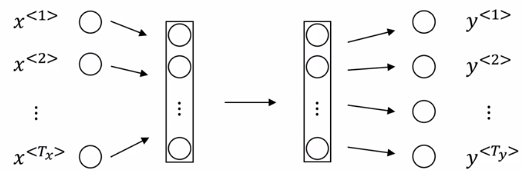
\includegraphics[scale=0.6]{1.png}
\end{figure}


事实上,这一方法存在的两个大问题使得这种传统的结构难以用来处理序列数据。
(1)不同样本的输入和输出往往具有不同的长度,我们可以对数据进行0填充或者1填充来使得数据之间的维度相适应,但这破坏了数据的原始结构,不是一个好的方法。(2)这样简单的网络结构不能够共享从数据的不同位置所得到的特征。比方说,当出现Harry时后面紧接着出现的单词很可能是一个人名,我们希望网络将这种学习到的信息进行共享,而这与卷积神经网络中的将图片中学习到的特征表示利用到其他图像类似。此外,通过权重共享也能够减少网络参数的规模。我们将要介绍的循环神经网络便能够克服这两个缺点。


一个简单的循环神经网络的前向传播过程如下所图所示:我们首先可以将第一个$a^{<0>}$初始化为零向量,然后进行前向传播过程,$a^{<1>}=g(W_{aa}a^{<0>}+b_a),\hat{y}^{<1>}=g(W_{ya}a^{<1>}+b_y)$,其中$W_{ax}$是将$x$变换成$a$的一个参数矩阵。隐藏层的激活函数通常选取tanh,但是有时也选取relu。输出层的激活函数根据不同的问题可选取不同类型的激活函数,例如分类问题中常常选取sigmoid或者softmax。

\begin{figure}[ht]
	\centering
	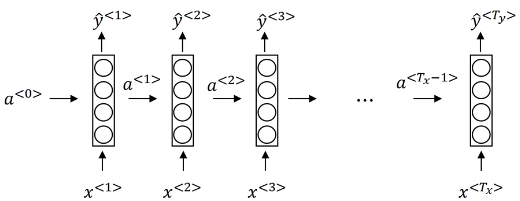
\includegraphics[scale=0.6]{2.png}
\end{figure}
在一般情形下,上述符号可以写为:
\begin{align*}
a^{<t>} &= g(W_{aa}a^{<t>}+W_{ax}x^{<t>}+b_a)\\
\hat{y}^{<t>}&=g(W_{ya}a^{<t>}+b_y)
\end{align*}
还可以将$W_{aa}$与$W_{ax}$合并从而得到更为精简的前向计算公式:
\begin{align*}
a^{<t>} &= g(W_{a}[a^{<t>},x^{<t>}]+b_a)\\
\hat{y}^{<t>}&=g(W_{y}a^{<t>}+b_y).
\end{align*}


一个基本的RNN模块如下图所示,该模块的输入是当前的输入$x^{<t>}$和由过去所有的隐藏状态累计下来的信息$a^{<t-1>}$,模块的输出是传入到下一个时刻的隐藏信息$a^{<t>}$和当前的预测信息$\hat{y}^{<t>}$。
\begin{figure}[htb!]
	\centering
	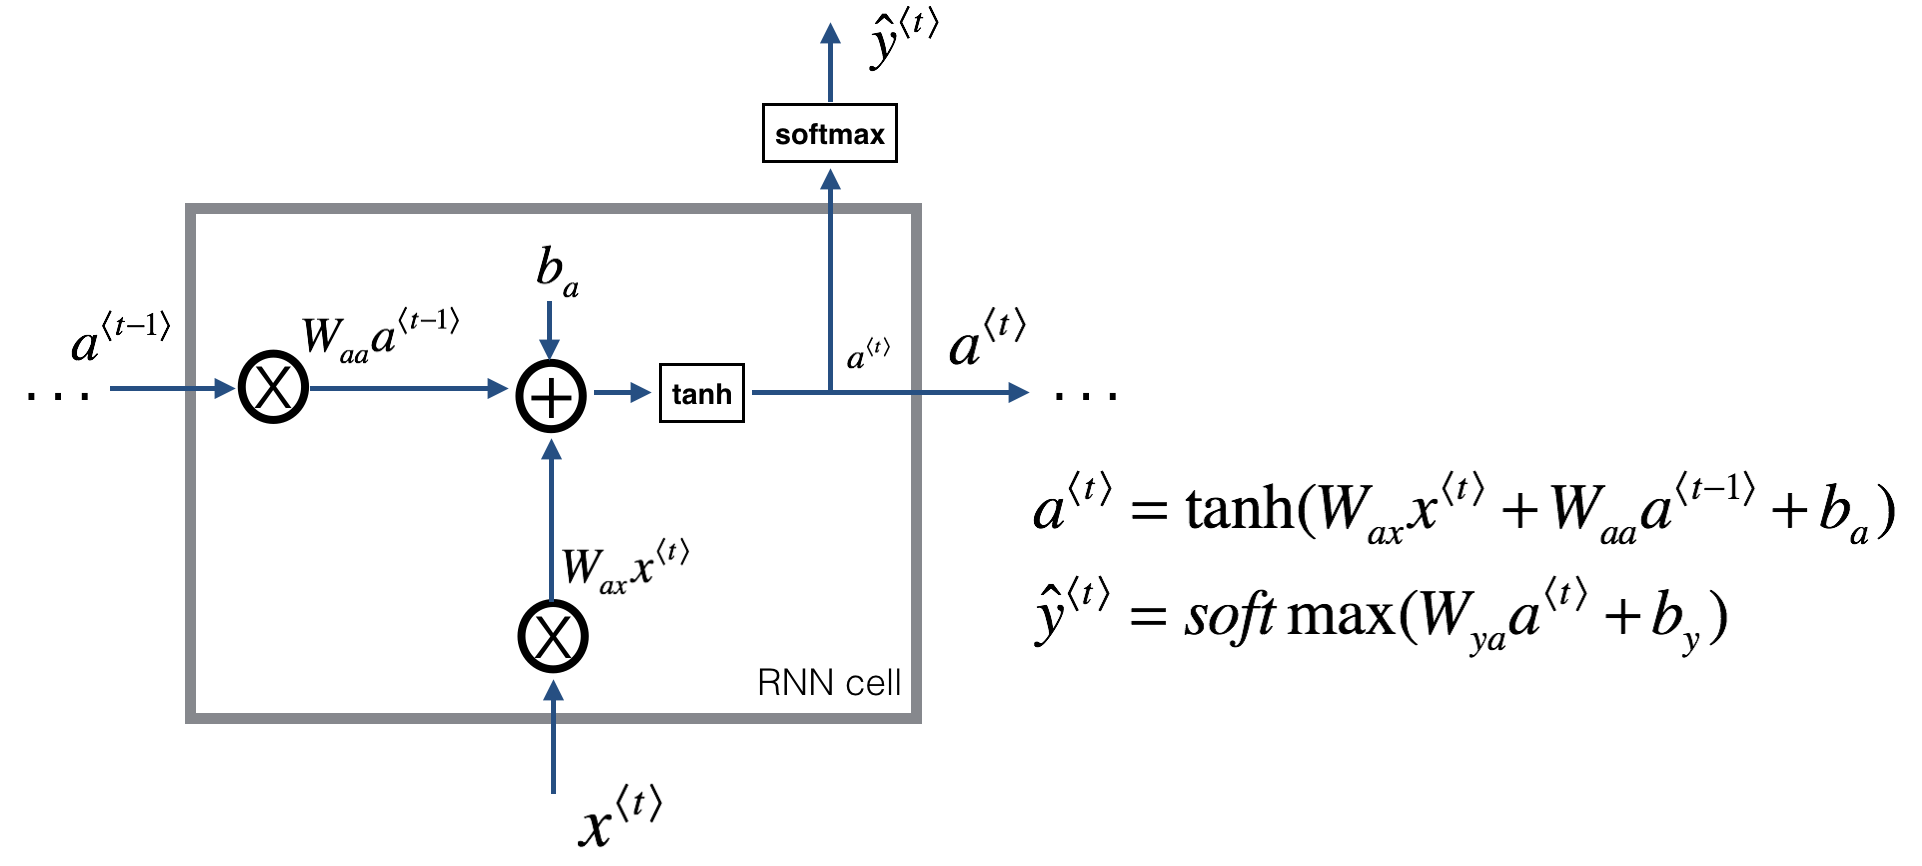
\includegraphics[scale=0.4]{rnn_step_forward.png}
\end{figure}
注意我们的样本总数为$m$,从而$x^{<t>}$的维数为$(n_x,m)$, $a^{t}$的维数为$(n_a,m)$, $W_{ax}$的维数为$(n_a,n_x)$, $W_{aa}$的维数为$(n_a,n_a)$, $W_{ya}$的维数为$(n_y,n_a)$。将上面的单个时间点的RNN模块展开,就可以得到如下的RNN基本表示:
\begin{figure}[htb!]
	\centering
	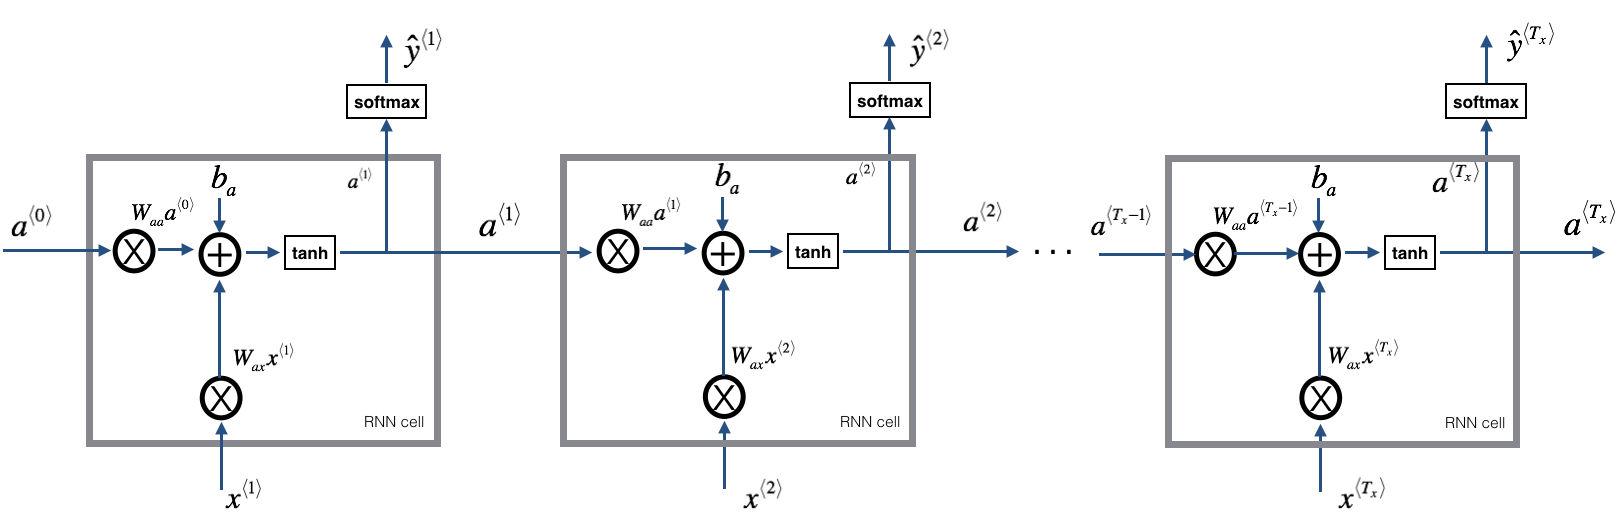
\includegraphics[scale=0.55]{rnn.png}
\end{figure}
\subsection{通过时间的反向传播}
RNN的反向传播过程的大致框架与传统的深度神经网络相同,需要注意的就是网络中的参数$W_a,b_a,W_y,b_y$是共享的。不失一般性,我们定义交叉熵损失作为我们的损失函数,即在单个输出上的损失可以定义为:
\begin{equation*}
\mathcal{L}{(\hat{y}^{<t>},y^{<t>})} = -y^{<t>}\log{\hat{y}^{<t>}}- (1-y^{<t>})\log{(1-\hat{y}^{<t>})}
\end{equation*}
于是损失函数的表达式为:
\begin{equation*}
\mathcal{J} = \sum_{t=1}^{T_y}\mathcal{L}{\left(\hat{y}^{<t>},y^{<t>}\right)}
\end{equation*}
隐藏层的激活函数我们选取$tanh$,于是单个基本块的前向传播过程可以具体写为如下表达式:
\begin{align*}
a^{<t>} &= tanh(W_{ax}x^{<t>}+W_{aa}a^{<t-1>}+b_a)\\
\hat{y}^{<t>} &= soft\max(W_{ya}a^{<t>}+b_y)
\end{align*}
反向传播的数据流图如下所示:
\begin{figure}[htb!]
	\centering
	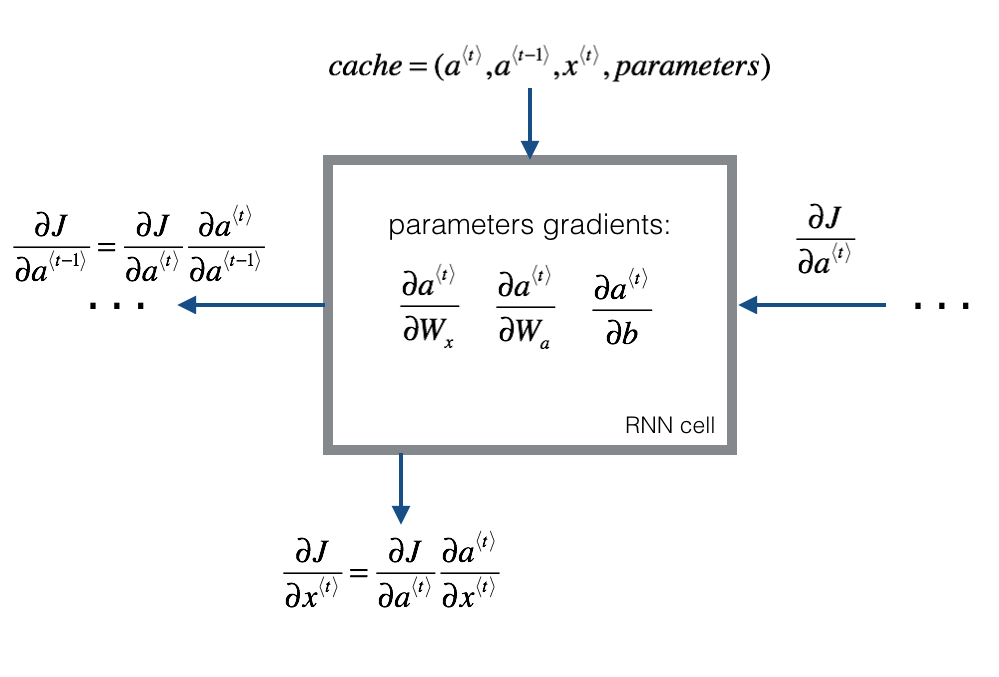
\includegraphics[scale=0.55]{rnn_cell_backprop.png}
\end{figure}


根据上面的数据流示意图,并结合$a^{<t>} = tanh(W_{ax}x^{<t>}+W_{aa}a^{<t-1>}+b_a),\frac{\partial{tanh(x)}}{\partial{x}}=1-tanh(x)^2$,我们可以写出单个RNN模块的反向传播过程的计算公式为:
\begin{align*}
\frac{\partial a^{<t>}}{\partial W_{ax}} &= (1-tanh(W_{ax}x^{<t>}+W_{aa}a^{<t-1>}+b_a)^2)x^{<t>T}\\
\frac{\partial a^{<t>}}{\partial W_{aa}} &= (1-tanh(W_{ax}x^{<t>}+W_{aa}a^{<t-1>}+b_a)^2)a^{<t-1>T}\\
\frac{\partial a^{<t>}}{\partial b_a} &= \sum_{batchsize}(1-tanh(W_{ax}x^{<t>}+W_{aa}a^{<t-1>}+b_a)^2)\\
\frac{\partial{a}^{<t>}}{\partial{x}^{<t>}} &= W_{ax}^T(1-tanh(W_{ax}x^{<t>}+W_{aa}a^{<t-1>}+b_a)^2)\\
\frac{\partial{a}^{<t>}}{\partial{a}^{<t-1>}} &= W_{aa}^T(1-tanh(W_{aa}x^{<t>}+W_{aa}a^{<t-1>}+b_a)^2)
\end{align*}
\subsection{循环神经网络的几种基本类型}
上面我们主要介绍了输入序列的长度$T_x$和输出序列的长度$T_y$相同的循环神经网络。事实上在实际应用中我们会遇到更多的RNN结构,比如:我们处理情感分类问题时的输出往往只有一个标量值,这时就是一个多对一的结构;音乐生成时使用的往往是一个一对多的网络结构,其有一个或者零个输入然后有多个输出;机器翻译任务中用到的网络结构是一个输入序列和输出序列长度不相等的多对多结构。
\subsection{小结}
到此我们便熟悉了循环神经网络的基本结构以及其前向计算过程和反向传播过程,由于其反向传播过程是从最后时刻一步步往前进行梯度传递的,因此这一过程常被称为通过时间的反向传播。后续的文章将对几种循环神经网络的结构如GRU和LSTM进行更为详细的介绍与公式推导。
\section{长短期记忆网络(LSTM)简介}
\subsection{长期依赖的问题}
循环神经网络的一个吸引人的地方在于其能够结合之前的状态保留下来的信息来用于当前任务的处理,比方说其可以利用视频文件中之前的帧所包含的信息来帮助理解当前的图像帧,或者根据句子中之前的文字信息来预测之后可能出现的单词。有时候我们只需考虑最近的信息来帮助解决当前的任务,比方说我们想要预测句子"The clouds are in the \textit{sky}."中的最后一个单词,我们只需要前面位置不远的几个词汇即可进行有效的预测; 而当我们面临下面这样的文本"I grew up in France… I speak fluent \textit{French}."来预测最后一个单词时,前面位置相近的词汇所能提供的信息或许只是最后的单词是一个语言的名字,若我们考虑更长的依赖关系我们便能够将这个范围缩小到"French"。LSTM就是针对数据的长短期依赖关系所提出的一个十分经典的循环神经网络结构,并且在自然语言处理,视频理解与目标检测,深度强化学习等领域有着十分广泛的应用。
\subsection{关于LSTM的一个直觉理解}
考虑这样一个场景,当我们在看一个精彩的电影时,我们会被电影中的各个精彩情节所吸引,但是我们不能够记住所有的电影情节。当观影结束时,我们会立马忘记电影里面一些无关紧要的情节,留在我们脑海中的可能更多的是一些对剧情发展起关键作用的场景,这些场景可能在之后的很长一段时间后依然停留在我们的脑海中,以至于当我们去观看电影的续集时还能够利用到之前所观看的电影的情节作为铺垫来帮助我们理解新的内容。人类的这一记忆过程可以抽象为对已有知识的选择性遗忘与选择性保留,事实上LSTM模块的设计便是与这一记忆过程有着十分密切的联系的。
\subsection{LSTM的基本结构}
LSTM与基本的递归神经网络具有类似的控制流程,不同的是LSTM基本单元内部的控制逻辑要稍稍复杂。LSTM的核心部件是基本单元,其中包含几个控制结构来对序列中的数据进行处理。LSTM基本块可以通过内部的门结构,包括遗忘门,更新门,输出门,来对之前的输入信息进行增加与遗忘,一个基本块内部基本单元之间的关系如下图所示。
\begin{figure}[htb!]
	\centering
	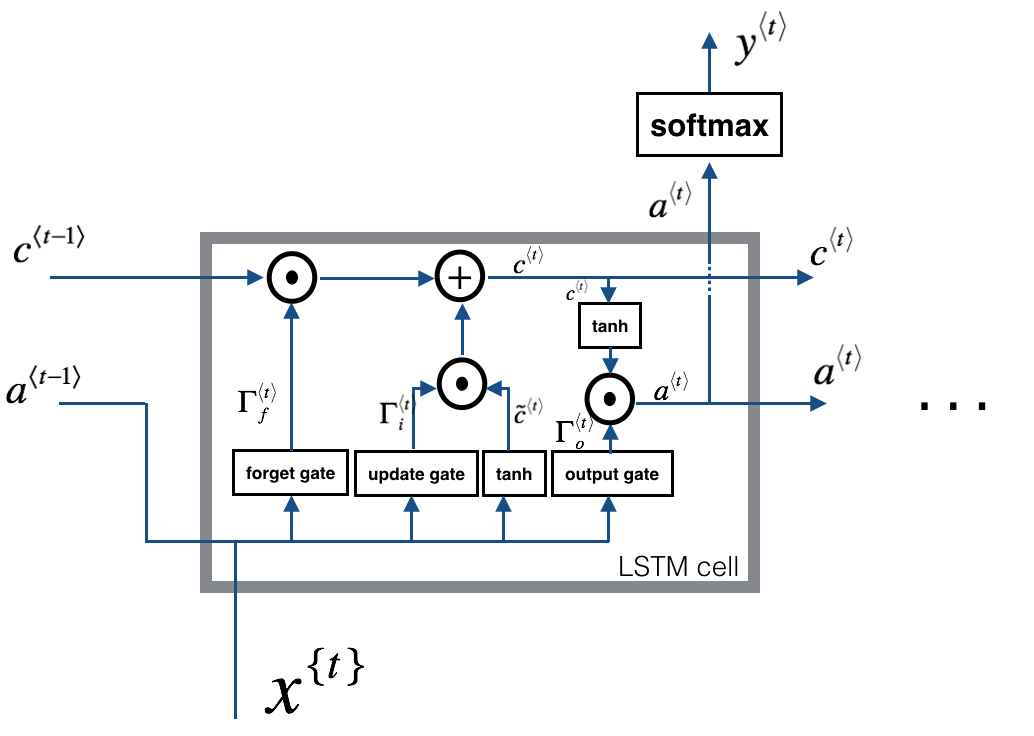
\includegraphics[scale=0.8]{LSTM.png}
\end{figure}
\subsubsection{遗忘门}
为了便于说明,我们可以用一个简单的例子来说明遗忘门所起的作用。假设我们用一个LSTM结构来跟踪一篇英文文本的语法结构,比方说主语的单复数,那么当文章的主语由单数变为复数的时候我们需要找到一个方法来清楚我们之前所保留的主语为单数的状态。在LSTM中,一个遗忘门结构执行如下的操作:
\begin{equation*}
\Gamma_f^{\langle t \rangle} = \sigma(W_f[a^{\langle t-1 \rangle}, x^{\langle t \rangle}] + b_f)
\end{equation*}
其中,$W_f$是用来控制遗忘门行为的权重矩阵,我们将$a^{\langle t-1 \rangle}$和$x^{\langle t \rangle}$连接起来并用$W_f$去乘连接后的矩阵,然后在加上一个偏置$b_f$,最后通过sigmoid函数将值映射到区间$[0,1]$。遗忘门的输出结果$\Gamma_f^{\langle t \rangle}$将会与上一个单元的状态值进行对应元素的乘法运算。因此,如果$\Gamma_f^{\langle t \rangle}$中的一个值为0或接近0,那么上一个单元$c^{\langle t-1 \rangle}$的对应信息(比方说代表主语为单数的信息)将被丢弃,如果$\Gamma_f^{\langle t \rangle}$中的值为1,那么对应的信息将被保留。
\subsubsection{更新门}
还是以跟踪句子主语的单复数为例,当我们在遗忘门中对主语为单数的状态信息进行遗忘后,还需要对状态进行更新写入以表明现在主语已经更新为复数了。更新门实际上就是在进行这一操作,其基本操作可表示为:
\begin{equation*}
\Gamma_u^{\langle t \rangle} = \sigma(W_f[a^{\langle t-1 \rangle}, x^{\langle t \rangle}] + b_u)
\end{equation*}
与遗忘门类似,更新门的输出结果$\Gamma_u^{\langle t \rangle}$同样是一个值在$[0,1]$范围内的向量。为了计算新的状态信息$c^{\langle t \rangle}$,更新门的输出结果将会与$\tilde{c}^{\langle t \rangle}$进行元素之间的乘法运算。
\subsubsection{单元状态的更新}
我们需要对在序列间进行传递的单元状态值$c$进行更新,如LSTM的结构图所示,首先我们需要计算中间变量为:
\begin{equation*}
\tilde{c}^{\langle t \rangle} = \tanh(W_c[a^{\langle t-1 \rangle}, x^{\langle t \rangle}] + b_c)
\end{equation*}
然后,新的单元状态为:
\begin{equation*}
c^{\langle t \rangle} = \Gamma_f^{\langle t \rangle}* c^{\langle t-1 \rangle} + \Gamma_u^{\langle t \rangle} *\tilde{c}^{\langle t \rangle}
\end{equation*}
我们可以看到,新的单元状态融合了过去的单元状态信息,旧的单元内部的隐藏信息以及新的输入数据。
\subsubsection{输出门}
输出门中可以得到当前单元的输出值$\Gamma_o^{\langle t \rangle}$和传递到下一个单元的隐藏状态值$a^{\langle t \rangle}$,其具体的计算过程如下:
\begin{align*}
\Gamma_o^{\langle t \rangle}&=  \sigma(W_o[a^{\langle t-1 \rangle}, x^{\langle t \rangle}] + b_o)\\
a^{\langle t \rangle} &= \Gamma_o^{\langle t \rangle}* \tanh(c^{\langle t \rangle})
\end{align*}
其中计算得到的$\Gamma_o^{\langle t \rangle}$可以根据需要接上一个sigmoid或者softmax作为网络单元的最后输出。
\subsubsection{RNN中的tanh函数}
我们知道一个向量被输入到神经网络之后会被执行很多的运算,tanh函数的图像如下所示,可以看出其将输入的向量变换到$(-1,1)$之间,这样当神经网络不断执行各种运算的时候就会在每一层对向量的值进行限制,从而避免出现向量内部各个值之间的差距过大的现象。当然传统的Relu也可用于RNN的激活函数,将RNN的激活函数变为Relu可能会产生很大的输出值,但是在这里我们不对RNN中激活函数的选择问题进行更加深入的探讨。
\begin{figure}[htb!]
	\centering
	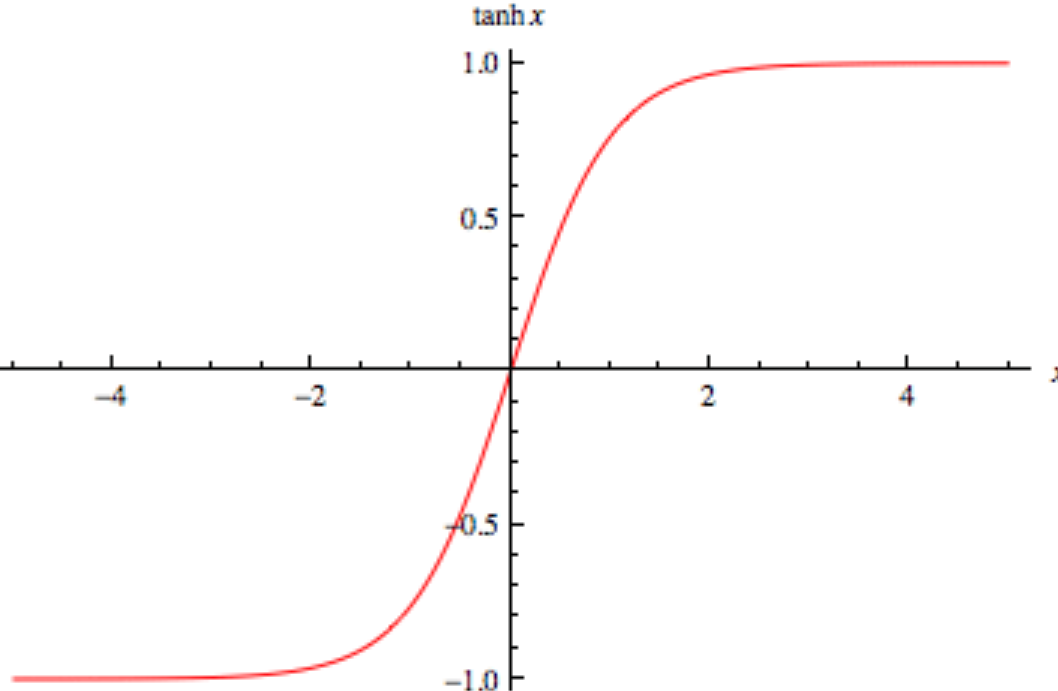
\includegraphics[scale=0.2]{tanh.png}
\end{figure}
\subsubsection{LSTM的前向传播过程}
根据上述的推导过程,我们便可得到如下的LSTM前向计算过程示意图:
\begin{figure}[htb!]
	\centering
	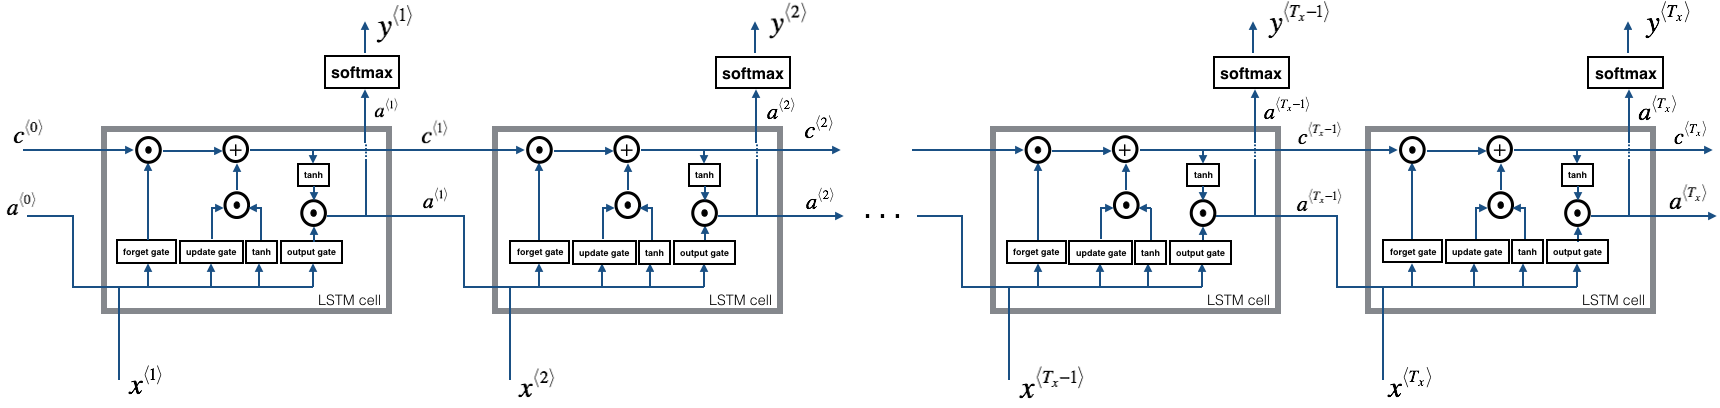
\includegraphics[scale=0.55]{LSTM_rnn.png}
\end{figure}
\subsection{LSTM的反向传播过程}
LSTM的反向传播过程较为复杂,需要特别注意的是单元内部的信息$c^{\langle t \rangle}$被前向传递到了$a^{\langle t \rangle}$和$c^{\langle t \rangle}$中,因此求导时链式法则涉及到$c^{\langle t \rangle}$的地方要特别注意。下面是LSTM单个单元反向传播过程的详细推导,注意在吴恩达深度学习作业中,该部分的过程有些小错误。
\begin{align*}
dW_o &= \frac{dJ}{dW_o}=\frac{dJ}{d\Gamma_o^{\langle t \rangle}}\frac{d\Gamma_o^{\langle t \rangle}}{dW_o}=\frac{dJ}{da_{\text{next}}}\frac{da_{\text{next}}}{d\Gamma_o^{\langle t \rangle}}\frac{d\Gamma_o^{\langle t \rangle}}{dW_o}\\&=da_{\text{next}}*tanh(c_{\text{next}})@\frac{d\Gamma_o^{\langle t \rangle}}{dW_o}\\
&=da_{\text{next}}*tanh(c_{\text{next}})*\Gamma_o^{\langle t \rangle}*(1-\Gamma_o^{\langle t \rangle})@\left(
\begin{matrix}
a_{\text{prev}}\\
x_t
\end{matrix}\right)^T\\
&\triangleq{d\Gamma_o^{\langle t \rangle}}@\left(
\begin{matrix}
a_{\text{prev}}\\
x_t
\end{matrix}\right)^T
\end{align*}
\begin{align*}
dW_f &= \frac{dJ}{dW_f}=\frac{dJ}{d\Gamma_f^{\langle t \rangle}}\frac{d\Gamma_f^{\langle t \rangle}}{dW_f}\\&=\left(dc_{\text{next}}*c_{\text{pre}}+\left(\Gamma_o^{\langle t\rangle}*(1-tanh(c_{\text{next}})^2)*da_{\text{next}}*c_{\text{pre}}\right)\right)*\left(\Gamma_f^{\langle t \rangle}*(1-\Gamma_f^{\langle t \rangle})\right)@\left(
\begin{matrix}
a_{\text{prev}}\\
x_t
\end{matrix}\right)^T\\
&=\left(dc_{\text{next}}+\left(\Gamma_o^{\langle t\rangle}*(1-tanh(c_{\text{next}})^2)*da_{\text{next}}\right)\right)*c_{\text{pre}}*\left(\Gamma_f^{\langle t \rangle}*(1-\Gamma_f^{\langle t \rangle})\right)@\left(
\begin{matrix}
a_{\text{prev}}\\
x_t
\end{matrix}\right)^T
\\
&\triangleq{d\Gamma_f^{\langle t \rangle}}@\left(
\begin{matrix}
a_{\text{prev}}\\
x_t
\end{matrix}\right)^T
\end{align*}
\begin{align*}
dW_u &= \frac{dJ}{dW_u}=\frac{dJ}{d\Gamma_u^{\langle t \rangle}}\frac{d\Gamma_u^{\langle t \rangle}}{dW_u}\\&=\left(dc_{\text{next}}*\tilde{c}^{\langle t \rangle}+\left(\Gamma_o^{\langle t\rangle}*(1-tanh(c_{\text{next}})^2)*da_{\text{next}}*\tilde{c}^{\langle t \rangle}\right)\right)*\left(\Gamma_u^{\langle t \rangle}*(1-\Gamma_u^{\langle t \rangle})\right)@\left(
\begin{matrix}
a_{\text{prev}}\\
x_t
\end{matrix}\right)^T\\
&=\left(dc_{\text{next}}+\left(\Gamma_o^{\langle t\rangle}*(1-tanh(c_{\text{next}})^2)*da_{\text{next}}\right)\right)*\tilde{c}^{\langle t \rangle}*\left(\Gamma_u^{\langle t \rangle}*(1-\Gamma_u^{\langle t \rangle})\right)@\left(
\begin{matrix}
a_{\text{prev}}\\
x_t
\end{matrix}\right)^T
\\
&\triangleq{d\Gamma_u^{\langle t \rangle}}@\left(
\begin{matrix}
a_{\text{prev}}\\
x_t
\end{matrix}\right)^T
\end{align*}
\begin{align*}
dW_c &= \frac{dJ}{dc^{\langle t \rangle}}\frac{dc^{\langle t \rangle}}{d\tilde{c}^{\langle t \rangle}}\frac{d\tilde{c}^{\langle t \rangle}}{dW_c}\\
&=\left(dc_{\text{next}}+\left(\Gamma_o^{\langle t\rangle}*(1-tanh(c_{\text{next}})^2)*da_{\text{next}}\right)\right)*\Gamma_u^{\langle t \rangle}*\left(1-(\tilde{c}^{\langle t \rangle})^2\right)@\left(
\begin{matrix}
a_{\text{prev}}\\
x_t
\end{matrix}\right)^T
\\
&\triangleq{d\tilde{c}^{\langle t \rangle}}@\left(
\begin{matrix}
a_{\text{prev}}\\
x_t
\end{matrix}\right)^T
\end{align*}
\begin{align*}
db_f &= np.sum(d\Gamma_f^{\langle t \rangle},axis=1,keepdims=True)\\
db_u &= np.sum(d\Gamma_u^{\langle t \rangle},axis=1,keepdims=True)\\
db_c &= np.sum(d\tilde{c}^{\langle t \rangle},axis=1,keepdims=True)\\
db_o &= np.sum(d\Gamma_o^{\langle t \rangle},axis=1,keepdims=True)\\
da_{prev} &= W_f^T[:,:,n_a]@d\Gamma_f^{\langle t \rangle} + W_u^T[:,:,n_a] @ d\Gamma_u^{\langle t \rangle}+ W_c^T[:,:,n_a] @ d\tilde c^{\langle t \rangle} + W_o^T[:,:,n_a] @ d\Gamma_o^{\langle t \rangle}\\
dc_{prev} &= dc_{next}*\Gamma_f^{\langle t \rangle} + \Gamma_o^{\langle t \rangle} * (1- \tanh(c_{next})^2)*\Gamma_f^{\langle t \rangle}*da_{next}\\
dx^{\langle t \rangle} &= W_f^T[:,n_a:]@d\Gamma_f^{\langle t \rangle} + W_u^T[:,n_a:] @ d\Gamma_u^{\langle t \rangle}+ W_c^T[:,n_a:] @ d\tilde c_t + W_o^T[:,n_a:] @ d\Gamma_o^{\langle t \rangle}
\end{align*}
\subsection{GRU与双向RNN}
GRU结构要比LSTM简单,在这里我们只给出其前向计算的计算过程:

\begin{align*}
\tilde{c}^{\langle t \rangle} &= tanh(W_c[\Gamma_r*c^{\langle t-1\rangle},x^{\langle t\rangle}] + b_c)\\
\Gamma_u &= \sigma(W_u[c^{\langle t-1\rangle},x^{\langle t\rangle}]+b_u)\\
\Gamma_r &= \sigma(W_r[c^{\langle t-1\rangle},x^{\langle t\rangle}]+b_c)\\
c^{\langle t\rangle} &= \Gamma_u*c^{\langle t\rangle} + (1-\Gamma_u)*c^{\langle t-1\rangle}
\end{align*}
其中$c^{\langle t\rangle}$作为单元的隐藏状态不断往后传递信息,同时在$c^{\langle t\rangle}$后加入sigmoid或者softmax函数作为当前单元的输出。可以明显的看出GRU具有比LSTM简单的结构,因此由于其计算代价较低,GRU在众多场合也有着十分广泛的应用。

上述提到的循环神经网络都能实现对过去的信息进行利用,我们考虑某个问题场景比如机器翻译问题知道未来的信息可能对当前的过程具有积极的作用,为了对序列数据中的当前时刻的未来信息加以利用,我们可以建立双向的RNN神经网络结构(BRNN)。BRNN的思路其实就是增加一个RNN模块,只不过这个模块的输入序列是正常序列数据的逆序,最后的输出结果是两个方向的输出进行汇总,从而达到同时利用过去的信息和未来的信息来解决当前问题的目的。

此外,我们还可以堆叠多个RNN模块,从而形成一个深度RNN结构,在Deep RNN 中,当前时刻的数据要经过多个RNN模块的前向计算才能得到最后的输出结果
\subsection{小结}
循环神经网络在处理序列化数据如语音识别,机器翻译等场景中具有非常广泛的应用,GRU和LSTM两种基本的结构通过模块中的门结构来控制信息的传递与利用,门结构也可视为对有用信息的一种提取方式。对数据中的有用数据进行抽取的新方法也在不断被提出,后续我们将对神经网络中的注意力机制进行介绍。
\end{document}